\documentclass{article}
\usepackage[%
    left=0.5in,%
    right=0.5in,%
    top=0.5in,%
    bottom=0.5in,%
]{geometry}%
\usepackage{minitoc}
\usepackage{multicol}
\usepackage{graphicx}
\usepackage{fixltx2e}
\usepackage{hyperref}
\usepackage{hyperref}
    \hypersetup{ colorlinks = true, linkcolor = blue }
\usepackage{blindtext}

\graphicspath{ {./} }

\newcommand{\inlinecode}[2]{\colorbox{lightgray}{\lstinline
[language=#1]$#2$}}
\newcommand{\worddef}[1]{\hyperref[sec:reference]{\textit{#1}}}

\begin{document}

\section{Memory}

\subsection{Models}
\begin{flushleft}
\textit{Contiguous memory} management models allocate memory in one single block without any holes or gaps.\\
\textit{Non-contiguous} memory management models are capable of allocating memory in multiple blocks, or segments, which may be placed anywhere in physical memory (i.e., not necessarily next to each other)
\end{flushleft}

\section{Partitioning}

\subsection{Overview}
\begin{itemize}
	\item Mono-programming: one single partition for user processes
	\item Multi-programming with fixed partitions
	\begin{itemize}
		\item Fixed equal sized partitions
		\item Fixed non-equal sized partitions 
	\end{itemize}
	\item Multi-programming with dynamic partitions
\end{itemize}

\subsection{Mono-Programming}
\begin{multicols}{2}

\begin{itemize}
	\item Only one single user process is in memory/executed at any point in time (no multi-programming)
	\item A \textbf{fixed region} of memory is allocated to the OS/kernel, the remaining memory is reserved for a single process (MS-DOS worked this way)
	\item This process has \textbf{direct} access to physical memory (i.e. no address translation takes place)
\end{itemize}

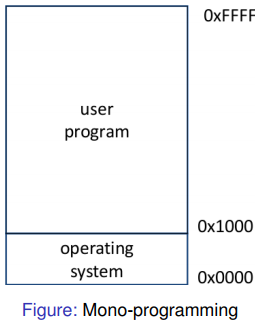
\includegraphics[scale=0.5]{Selection_001.png}
\end{multicols}

\begin{itemize}
	\item Every process is allocated \textbf{contiguous block of memory}, i.e. it contains no “holes” or “gaps” (⇔ non-contiguous allocation)
	\item One process is allocated the \textbf{entire memory space}, and the process is \textbf{always} located in the same address space.
	\item \textbf{No protection} between different user processes required (one process).
	\item \textbf{Overlays} enable the programmer to use more memory than available (burden on programmer)
\end{itemize}

\subsubsection{Shortcomings}
\begin{flushleft}
\begin{itemize}
	\item Since a process has \textbf{direct} access to the physical memory, it may have access to OS memory.
	\item The operating system can be seen as a process - so we have two processes anyway
	\item \textbf{Low utilisation} of hardware resources (CPU, I/O devices, etc.)
	\item Mono-programming is \textbf{unacceptable} as multiprogramming is expected on modern machines
\end{itemize}
\bigskip
Direct memory access and mono-programming are \textbf{common in basic embedded systems} and modern consumer electronics, e.g. washing machines, microwaves, car’s ECUs, etc.
\end{flushleft}

\pagebreak
\subsection{Multi-programming}
\begin{flushleft}
Simulate multi-programming through swapping: 
\begin{itemize}
	\item Swap process out to the disk and load a new one (context switches would become time consuming)
	\item Apply threads within the same process (limited to one process)
\end{itemize}
To calculate \textit{CPU utilisation}
\begin{itemize}
	\item There are $n$ processes in memory
	\item A process spends $p$ percent of its time waiting for I/O
	\item The CPU utilisation is given by $ 1 - (p^n) $
\end{itemize}
Multi-programming does \textbf{enable to improve} resource utilisation \verb!->! memory management should provide support for multi-programming.\\
\textbf{Caveats}:\\
\begin{itemize}
	\item This model assumes that all processes are \textbf{independent}, this is not true
	\item More complex models could be built using \textit{theory}, but we can still use this simplistic model to make approximate predictions
\end{itemize}
\end{flushleft}

\subsection{Partitioning methods}
\subsubsection{Fixed Partitions of equal size}
\begin{flushleft}
Divide memory into \textbf{static, contiguous and equal sized partitions} that have a \textbf{fixed size} and \textbf{fixed location}
\begin{itemize}
	\item Any process can take \textbf{any} (large enough) partition
	\item Allocation of \textbf{fixed equal sized} partitions to processes is trivial
	\item \textbf{Very little overhead} and simple implementation The OS keeps a track of which partitions are being used and which are free
\end{itemize}
\textbf{Disadvantages}:
\begin{itemize}
	\item \textbf{Low memory utilisation} and internal fragmentation: partition may be unnecessarily large
	\item Overlays must be used if a program does not fit into a partition (burden on programmer)
\end{itemize}
\end{flushleft}

\subsubsection{Fixed Partitions of non-equal size}
\begin{flushleft}
Divide memory into static and \textbf{non-equal} sized partitions that have a \textbf{fixed size} and \textbf{fixed location}
\begin{itemize}
	\item Reduces internal fragmentation
	\item The allocation of processes to partitions must be carefully considered
\end{itemize}
\end{flushleft}

\subsubsection{Fixed partition allocation methods}
\begin{flushleft}
\textbf{One private} queue per partition:
\begin{itemize}
	\item Assigns each process to the \textbf{smallest partition} that it would fit in
	\item Reduces internal fragmentation
	\item Can reduce memory utilisation (e.g., lots of small jobs result in unused large partitions) and result in starvation 
\end{itemize}
A \textbf{single shared queue} for all partitions can allocate small processes to large partitions but results in increased \textit{internal fragmentation}
\end{flushleft}
\end{document}
